\documentclass[a4paper,12pt]{article} 
%%%%%%%%%%%%%%%%%%%%%%%%%%%%%%%% CONSTANTES %%%%%%%%%%%%%%%%%%%%%%%%%%%%%%%%%%%
\newcommand{\numero}{10}                                    %Numéro de la série -1

\usepackage[french]{babel}
\usepackage[utf8]{inputenc}
\usepackage{answers}

\usepackage{hyperref}
\usepackage{multicol}

\usepackage[table,xcdraw]{xcolor}
\usepackage{listings}
\definecolor{ForestGreen}{RGB}{34,139,34}


\usepackage{enumitem}

\AtBeginDocument{\def\labelitemi{$\bullet$}}


\newcommand{\py}{\lstinline{Python} }


\definecolor{backcolour}{rgb}{0.95,0.95,0.92}

\lstset{%
	language         = Python,
	backgroundcolor  = \color{backcolour},
	basicstyle       = \ttfamily, % \upshape\ttfamily,
	keywordstyle     = \bfseries\color{blue}, %\bfseries,
	stringstyle      = \color{magenta},
	commentstyle     = \color{ForestGreen},
	alsoletter = > ,
	morekeywords = {>>>,as,assert,False,None, nonlocal,True, with,yield , <<, >>, :},
	showstringspaces = false,
	numbers=left,
	stepnumber=1,
	literate={à}{{\`{a}}}1 {é}{{\'e}}1 {è}{{\`{e}}}1 {ê}{{\^{e}}}1 {Ê}{{\^{E}}}1 {î}{{\^i}}1 {ô}{{\^{o}}}1 {ç}{{\c{c}}}1 {Ç}{{\c{C}}}1
}

\newcommand{\itemb}[1]{\item \textbf{#1}}

\usepackage{fancyhdr}  %package pour en-tetes et pied de pages
\usepackage{sectsty} % Permet de faire des modifications de police dans diverses sections des "headings" (cf. modif presentation de la page)
\pagestyle{fancy}       %Style pour en-tetes et pieds de pages
\fancyhead[CO,CE]{\sc Série 1\hspace{0.5mm}}
\fancyhead[RO,LE]{Collège Sismondi}  % LaTeX/TEX define \strut to be an invisible box of width zero that extends just enough above and below the baseline. Cela permet d'augementer légèrement la taille en bas de la box de manière à ce qu'elle soit collée à la ligne.
\fancyhead[LO,RE]{\small\ \textsl{1\textsuperscript{ère} année - DO Informatique}}
\fancyfoot[RO,LE]{2021 - 2022}
\fancyfoot[LO,RE]{\small }
\fancyfoot[CO,CE]{\thepage}

\fancyhfoffset[l]{1.2cm} % le "l" en paramètre permet d'indiquer qu'on ne veut modifier que la marge à gauche.
\renewcommand{\headrule}{{%
		\hrule \headwidth \headrulewidth \vskip-\headrulewidth}}
\renewcommand\footrulewidth{\headrulewidth}
\renewcommand{\footrule}{{%
		\vskip-\footruleskip\vskip-\footrulewidth
		\hrule \headwidth \footrulewidth\vskip\footruleskip}}

\usepackage{tikz}
%-------------------------------------------------------------------------------
%---- Eclairage : en encadré sur fond jaune avec symbôle "ampoule" à gauche ----
%-------------------------------------------------------------------------------
\definecolor{coleclairage}{RGB}{255 , 221 , 156}
\definecolor{contoureclairage}{RGB}{255 , 192 , 0}
\newenvironment{eclairage}
{
	\begin{center}%
		\begin{tikzpicture}%
			\node[rectangle, draw=contoureclairage, top color=coleclairage!50, bottom color=coleclairage!140, rounded corners=5pt, inner xsep=5pt, inner ysep=6pt, outer ysep=10pt]\bgroup                     
			\begin{minipage}{0.98\linewidth}
				\begin{minipage}{0.08\linewidth}\centerline{
\includegraphics[scale=1]{Symbole_eclairage.png}}\end{minipage}
				\begin{minipage}{0.89\linewidth}\itshape\footnotesize
				}
				{                		
				\end{minipage}
			\end{minipage}\egroup;%
		\end{tikzpicture}%
	\end{center}%
}

%-------------------------------------------------------------------------------
%---- apprendre : en encadré sur fond jaune avec symbôle "ampoule" à gauche ----
%-------------------------------------------------------------------------------
\definecolor{colapprendre}{RGB}{50,205,50}
\definecolor{contourapprendre}{RGB}{34,139,34}
\newenvironment{apprendre}
{
	\begin{center}%
		\begin{tikzpicture}%
			\node[rectangle, draw=contourapprendre, top color=colapprendre!10, bottom color=colapprendre!50, rounded corners=5pt, inner xsep=5pt, inner ysep=6pt, outer ysep=10pt]\bgroup                     
			\begin{minipage}{0.98\linewidth}
				\begin{minipage}{0.08\linewidth}\centerline{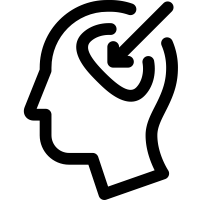
\includegraphics[width=30px]{Symbole_learn.png}}\end{minipage}
				\begin{minipage}{0.89\linewidth}\itshape\footnotesize
				}
				{                		
				\end{minipage}
			\end{minipage}\egroup;%
		\end{tikzpicture}%
	\end{center}%
}

\definecolor{colimportant}{RGB}{247 , 189 , 164}
\definecolor{contourimportant}{RGB}{237 , 125 , 49}
\newenvironment{important}
{
	\begin{center}%
		\begin{tikzpicture}%
			\node[rectangle, draw=contourimportant, top color=colimportant!50, bottom color=colimportant!140, rounded corners=5pt, inner xsep=5pt, inner ysep=6pt, outer ysep=10pt]\bgroup                     
			\begin{minipage}{0.08\linewidth}\centerline{
\includegraphics[scale=0.8]{Symbole_attention.png}}\end{minipage}
			\begin{minipage}{0.89\linewidth}
			}
			{                		
			\end{minipage}\egroup;
		\end{tikzpicture}%
	\end{center}%
}

%-----------------------------------------------------------------
%---- Modification présentation de la page: marges de la page ----
%-----------------------------------------------------------------
%\addtolength{\hoffset}{-1in}              % 1
%\addtolength{\voffset}{-1in}              % 2
\addtolength{\oddsidemargin}{-0.1 in} % 3
\addtolength{\evensidemargin}{-1in} % 3
\addtolength{\topmargin}{-1in}       % 4
\addtolength{\headheight}{6pt}       % 5
%\addtolength{\headsep}{-0.2cm}           % 6
\setlength{\textheight}{26cm}    % 7
\setlength{\textwidth}{16.5cm}      % 8
\addtolength{\marginparsep}{0pt}      % 9
\setlength{\marginparwidth}{0pt}   % 10
\addtolength{\footskip}{-1mm}           %11

\setlength{\parindent}{0em}% pas d'indentation


% Customiser le nom des sections
\usepackage{titlesec}
\titleformat{\section}[hang]{\Large \bfseries}{Série \thesection:\ }{0pt}{}

\renewcommand{\familydefault}{\sfdefault} % pour avoir des polices san serif

\newtheorem{Exc}{Exercice}
\Newassociation{correction}{Soln}{mycor}
\renewcommand{\Solnlabel}[1]{\bfseries Ex #1 }
\def\exo#1{%
	\futurelet\testchar\MaybeOptArgmyexoo}
\def\MaybeOptArgmyexoo{
	\ifx[\testchar \let\next\OptArgmyexoo
	\else \let\next\NoOptArgmyexoo \fi \next}
\def\OptArgmyexoo[#1]{%
	\begin{Exc}[#1]\normalfont}
	\def\NoOptArgmyexoo{%
		\begin{Exc}\normalfont}
		\newcommand{\finexo}{\end{Exc} \vspace{3mm}}
	\newcommand{\flag}[1]{}
	\newcommand{\entete}[1]

\newcommand{\getexocompteur}{{\the\numexpr \arabic{Exc}  \relax}}	
	
\newcommand{\eexo}{\vspace{5mm}} % espace pour séparer les exercices

\begin{document}
%		\title{\vspace{-3cm}Série 1}
%		\date{\vspace{-2cm}}
%		\maketitle

\fancyhead[CO,CE]{\sc Série \arabic{section} \hspace{0.5mm}}

\setcounter{section}{\numero}
\section{Les séquences et les boucles for}				
\Opensolutionfile{mycor}[cor_01]

\exo[Quelle boucle choisir]{}  ~\\ 
Quelle boucle est adaptée à l’écriture de programmes traitant les problèmes suivants :
\begin{enumerate}
	\item le calcul du total à payer à une caisse enregistreuse,
	\item la recherche du jour le plus pluvieux d’une année,
	\item le calcul du périmètre d’un polygone,
	\item le calcul de la durée d’une émission de radio, connaissant ses horaires de début et de fin ?
\end{enumerate}
\begin{correction}
	~\\ 
	\begin{enumerate}
		\item   Une boucle \lstinline!while! : on ne sait pas combien il y aura d’articles, on ne s’arrête que lorsque le tapis est vide.
		\item Une boucle \lstinline!for! : le corps de la boucle doit être répété 365 fois exactement.
		\item Cela dépend : si le nombre de côtés est connu, une boucle \lstinline!for! , sinon, une boucle \lstinline!while! qui s’arrête lorsqu’on est revenu au sommet de départ.
		\item Il n’y a pas besoin de boucle.
	\end{enumerate}
\end{correction}
\finexo


\exo{}  ~\\ 
\begin{enumerate}[label=\alph*)]
	\item Écrire un programme qui, étant donnés deux bornes entières a et b données en entrée par l’utilisateur, additionne les multiples de 3 et 5 compris entre ces bornes. Ainsi, pour a = 0 et b = 32, le résultat doit être 0 + 15 + 30 = 45.
	\item Modifier légèrement le programme précédent pour qu’il additionne les multiples de 3 ou 5 compris entre les bornes a et b. Ainsi, pour a = 0 et b = 32, le résultat doit être 0 + 3 + 5 + 6 + 9 + 10 + 12 + 15 + 18 + 20 + 21 + 24 + 25 + 27 + 30 = 225
\end{enumerate}
\begin{correction}
	~\\ 
	\begin{enumerate}[label=\alph*)]
		\item \lstinputlisting[numbers=none]{codes/ex2_corrige_a.py}
		
		\item  \lstinputlisting[numbers=none]{codes/ex2_corrige_b.py}
	\end{enumerate}


\end{correction}
\finexo

\exo{}  ~\\ 
	Écrire un programme qui détermine le plus petit multiple commun à deux nombres entiers entrés au clavier.
	\begin{correction}
		~\\ 
		\lstinputlisting[numbers=none]{codes/ex3_corrige.py}
	\end{correction}
\finexo


\exo{}  ~\\ 
Écrire un script qui prend en entrée une chaîne de caractères et retourne en sortie une copie de la chaîne entrée après avoir inséré un astérisque entre tous les caractères. 
Exemple : \texttt{gaston} devra donner \texttt{g*a*s*t*o*n}.
\begin{correction}
	~\\ 
	\lstinputlisting[numbers=none]{codes/ex4_corrige.py}
\end{correction}
\finexo


\exo{}  ~\\ 
Écrire un programme qui prend en entrée une chaîne de caractères et retourne en sortie une copie de la chaîne entrée après avoir inversé l’ordre des caractères qui la composent. 
Exemple : gaston devra donner notsag.
\begin{correction}
	~\\ 
	\lstinputlisting[numbers=none]{codes/ex5_corrige.py}
\end{correction}
\finexo



\exo{}  ~\\ 
Une balle rebondissante est lâchée du haut d'un immeuble de 10 mètres. A chaque rebond la hauteur diminue d'un tiers. Combien de fois la personne du premier niveau dont la fenêtre est située à 1 mètre 50 du sol verra elle passer la balle ? 
\begin{correction}
	~\\ 
	\lstinputlisting[numbers=none]{codes/ex6_corrige.py}
\end{correction}
\finexo


\exo{}  ~\\ 
Un triplet pythagoricien est un ensemble de trois entiers (a, b, c) pouvant représenter les trois côtés d’un triangle rectangle c’est-à-dire vérifiant l’égalité $c^2 = a^2 + b^2$ . Écrire un programme qui génère tous les triplets pythagoriciens (sans doublon) où $a$, $b$ et $c$ sont inférieurs à 50.
\begin{correction}
	~\\ 
		\lstinputlisting[numbers=none]{codes/ex7_corrige.py}
\end{correction}
\finexo


\exo{}[Apprendre en  autonomie avec france IOI]  ~\\ 
Allez sur le site de france IOI sur \url{http://www.france-ioi.org/}, puis valider la séquence 2 (Niveau 2) :  "\textit{2 – Découverte des tableaux}".
\finexo

\exo{}  ~\\ 
Pour une valeur initial $u_0$, on définit la suite de Syracuse de $u_0$ de la manière suivante :
\begin{itemize}
	\item si $u_n = 1$, alors la suite est finie et un est son dernier élément (on arrête de calculer d’autres éléments)
	\item si $u_n$ est pair, alors $u_n+1  = u_n / 2$
	\item si $u_n$ est impair et distinct de 1, alors $u_n+1 = 3 u_n + 1$
\end{itemize}
Écrire un programme qui affiche les termes de la suite $\{u_k\}$.
Cette suite est-elle finie ?
Pour aller plus loin, aller vous renseigner sur la Conjecture de Syracuse1.\\

.
\begin{correction}
	~\\ 
	\lstinputlisting[numbers=none]{codes/ex9_corrige.py}
\end{correction}

\finexo

\cleardoublepage


% Solution		
		\newpage
		\setcounter{page}{1}
		\setcounter{section}{\numero}
		\Closesolutionfile{mycor}
		\titleformat{\section}[hang]{\Large \bfseries}{Corrigé Série \thesection:\ }{0pt}{}
		

		\fancyhead[CO,CE]{\sc Corrigé Série \arabic{section} \hspace{0.5mm}}
		\section{}
		\Readsolutionfile{mycor}
	\end{document}